\documentclass[10pt,a4paper,onecolumn]{article}
% \usepackage[utf8]{inputenc}
\usepackage{marginnote}
\usepackage{graphicx}
\usepackage{xcolor}
\usepackage{authblk,etoolbox}
\usepackage{titlesec}
\usepackage{calc}
\usepackage{hyperref}
\hypersetup{breaklinks=true,
            bookmarks=true,
            pdfauthor=
{
      Owen Petchey,
      Marco Plebani,
      Frank Pennekamp,
  },
            pdftitle=
{
[Re] Chaos in a long-term experiment with a plankton community
},
            colorlinks=true,
            citecolor=blue,
            urlcolor=blue,
            linkcolor=blue,
            pdfborder={0 0 0}}
\urlstyle{same}
\usepackage{tcolorbox}
\usepackage{ragged2e}
\usepackage{fontspec}
\usepackage{fontawesome}
\usepackage{caption}
\usepackage{listings}
\lstnewenvironment{code}{\lstset{language=Haskell,basicstyle=\small\ttfamily}}{}



%\usepackage{fancyvrb}
%\VerbatimFootnotes
%\usepackage{graphicx}
%\usepackage{mdframed}
%\newmdenv[backgroundcolor=lightgray]{Shaded}


\usepackage{longtable,booktabs}

\usepackage[
  backend=biber,
%  style=alphabetic,
%  citestyle=numeric
]{biblatex}
\bibliography{article.bib}



% --- Macros ------------------------------------------------------------------
\renewcommand*{\bibfont}{\small \sffamily}

\definecolor{red}{HTML}{CF232B}
\newcommand{\ReScience}{Re{\bfseries \textcolor{red}{Science}}}

\newtcolorbox{rebox}
   {colback=blue!5!white, colframe=blue!40!white,
     boxrule=0.5pt, arc=2pt, fonttitle=\sffamily\scshape\bfseries,
     left=6pt, right=20pt, top=6pt, bottom=6pt}

\newtcolorbox{repobox}
   {colback=red, colframe=red!75!black,
     boxrule=0.5pt, arc=2pt, left=6pt, right=6pt, top=3pt, bottom=3pt}

% fix for pandoc 1.14     
\newcommand{\tightlist}{%
  \setlength{\itemsep}{1pt}\setlength{\parskip}{0pt}\setlength{\parsep}{0pt}}

% --- Style -------------------------------------------------------------------
\renewcommand*{\bibfont}{\small \sffamily}
\renewcommand{\captionfont}{\small\sffamily}
\renewcommand{\captionlabelfont}{\bfseries}

\makeatletter
\renewcommand\@biblabel[1]{{\bf #1.}}
\makeatother

% --- Page layout -------------------------------------------------------------
\usepackage[top=3.5cm, bottom=3cm, right=1.5cm, left=1.5cm,
            headheight=2.2cm, reversemp, includemp, marginparwidth=4.5cm]{geometry}

% --- Section/SubSection/SubSubSection ----------------------------------------
\titleformat{\section}
  {\normalfont\sffamily\Large\bfseries}
  {}{0pt}{}
\titleformat{\subsection}
  {\normalfont\sffamily\large\bfseries}
  {}{0pt}{}
\titleformat{\subsubsection}
  {\normalfont\sffamily\bfseries}
  {}{0pt}{}
\titleformat*{\paragraph}
  {\sffamily\normalsize}


% --- Header / Footer ---------------------------------------------------------
\usepackage{fancyhdr}
\pagestyle{fancy}
%\renewcommand{\headrulewidth}{0.50pt}
\renewcommand{\headrulewidth}{0pt}
\fancyhead[L]{\hspace{-1cm}
\includegraphics[width=4.0cm]{rescience-logo.pdf}}
\fancyhead[C]{}
\fancyhead[R]{} 
\renewcommand{\footrulewidth}{0.25pt}

\fancyfoot[L]{\hypersetup{urlcolor=red}
              \sffamily \ReScience~$\vert$
              \href{http://rescience.github.io}{rescience.github.io}
              \hypersetup{urlcolor=blue}}
\fancyfoot[C]{\sffamily \thepage}
\fancyfoot[R]{\sffamily Sep 2015 $\vert$
                        Volume \textbf{1} $\vert$
                        Issue \textbf{1}}
\pagestyle{fancy}
\makeatletter
\let\ps@plain\ps@fancy
\fancyheadoffset[L]{4.5cm}
\fancyfootoffset[L]{4.5cm}

% --- Title / Authors ---------------------------------------------------------
% patch \maketitle so that it doesn't center
\patchcmd{\@maketitle}{center}{flushleft}{}{}
\patchcmd{\@maketitle}{center}{flushleft}{}{}
% patch \maketitle so that the font size for the title is normal
\patchcmd{\@maketitle}{\LARGE}{\LARGE\sffamily}{}{}
% patch the patch by authblk so that the author block is flush left
\def\maketitle{{%
  \renewenvironment{tabular}[2][]
    {\begin{flushleft}}
    {\end{flushleft}}
  \AB@maketitle}}
\makeatletter
\renewcommand\AB@affilsepx{ \protect\Affilfont}
%\renewcommand\AB@affilnote[1]{{\bfseries #1}\hspace{2pt}}
\renewcommand\AB@affilnote[1]{{\bfseries #1}\hspace{3pt}}
\makeatother
\renewcommand\Authfont{\sffamily\bfseries}
\renewcommand\Affilfont{\sffamily\small\mdseries}
\setlength{\affilsep}{1em}

\LetLtxMacro{\OldIncludegraphics}{\includegraphics}
\renewcommand{\includegraphics}[2][]{\OldIncludegraphics[width=12cm, #1]{#2}}


% --- Document ----------------------------------------------------------------
\title{[Re] Chaos in a long-term experiment with a plankton community}

    \usepackage{authblk}
                        \author[1]{Owen Petchey}
                    \author[1]{Marco Plebani}
                    \author[1]{Frank Pennekamp}
                            \affil[1]{Department of Evolutionary Biology and Environmental Studies, University
of Zurich, Zurich, Switzerland}
            
\date{\vspace{-5mm}
      \sffamily \small \href{mailto:owen.petchey@ieu.uzh.ch}{owen.petchey@ieu.uzh.ch}}


\setlength\LTleft{0pt}
\setlength\LTright{0pt}


\begin{document}
\maketitle

\marginpar{
  %\hrule
  \sffamily\small
  %\vspace{2mm}
  {\bfseries Editor}\\
  Name Surname\\

  {\bfseries Reviewers}\\
        Name Surname\\
        Name Surname\\
  
  {\bfseries Received}  Sep, 1, 2015\\
  {\bfseries Accepted}  Sep, 1, 2015\\
  {\bfseries Published} Sep, 1, 2015\\

  {\bfseries Licence}   \href{http://creativecommons.org/licenses/by/4.0/}{CC-BY}

  \begin{flushleft}
  {\bfseries Competing Interests:}\\
  The authors have declared that no competing interests exist.
  \end{flushleft}

  \hrule
  \vspace{3mm}

  \hypersetup{urlcolor=white}
  
    \vspace{-1mm}
  \begin{repobox}
    \bfseries\normalsize
      \href{https://github.com/opetchey/ReScience-submission/tree/petchey-plebani-pennekamp-2016/article}{\faGithubAlt~Article repository}
  \end{repobox}
      \vspace{-1mm}
  \begin{repobox}
    \bfseries\normalsize
      \href{https://github.com/opetchey/ReScience-submission/tree/petchey-plebani-pennekamp-2016/code}{\faGithubAlt~Code repository}
  \end{repobox}
      \vspace{-1mm}
  \begin{repobox}
    \bfseries\normalsize
      \href{https://github.com/opetchey/ReScience-submission/tree/petchey-plebani-pennekamp-2016/data}{\faGithubAlt~Data repository}
  \end{repobox}
      \hypersetup{urlcolor=blue}
}

\begin{rebox}
\sffamily {\bfseries A reference implementation of}
\small
\begin{flushleft}
\begin{itemize}
    \item[→] Benincà, E., Huisman, J., Heerkloss, R., Jöhnk, K.D., Branco, P., Van
Nes, E.H., Scheffer, M. \& Ellner, S.P. (2008) Chaos in a long-term
experiment with a plankton community. Nature, 451, 822--825 DOI:
10.1038/nature06512
  \end{itemize}\par
\end{flushleft}
\end{rebox}


\section{Draft article}\label{draft-article}

\section{Introduction}\label{introduction}

The original paper describes analyses of fluctuations in the abundance
of organisms in a plankton community derived from the Baltic Sea, housed
in a laboratory environment. The length of the time series (samples
every few days for 2,300 days) allowed for analyses revealing that the
observed dynamics exhibited characteristics consistent with chaos
produced by non-linear species interactions. The article concludes that
stability is not required for persistence of complex food webs, and that
long-term prediction of abundances may be fundamentally impossible. The
demonstration of chaotic dynamics and limited forecast horizons (sensu
\textcite{Petchey2015}) is important in the field of ecology, since the
ability to predict dynamics is an open question with considerable
applied importance (\textcite{Petchey2015} \textcite{Mouquet2015}.)

\section{Methods}\label{methods}

This reproduction started with the raw data (source given below) and
used information from the original paper,
\href{http://www.nature.com/nature/journal/v451/n7180/extref/nature06512-s1.pdf}{the
supplement to the original paper}, and communications with Elisa
Benincà, who provided for comparison digitised data from the original
article, and Stephen Ellner, who provided code and data used to produce
results in the original paper. Use of this data and code in this
reproduction is indicated below.

\subsection{Scope of the reproduction}\label{scope-of-the-reproduction}

An attempt was made to reproduce the majority of the results in the
original article. Instances where we did not attempt to reproduce a
result are detailed below.

\subsection{The data}\label{the-data}

The data are available as an Excel file supplement to
\href{http://onlinelibrary.wiley.com/doi/10.1111/j.1461-0248.2009.01391.x/abstract}{an
Ecology Letters publication} (\textcite{Beninca2009}). The Excel file
contains several datasheets. Two were particularly important, as they
were the source of the raw data (one contains original species
abundances, the other the nutrient concentrations). We saved these two
datasheets, without any alteration, as comma separated value (csv) text
files. In the code associated with this reproduction, these data files
are read from the associated github repository. Another datasheet
contained transformed data (we also saved this as csv file, in order to
use it in this reproduction). We also received a dataset direct from
Steve Ellner, see below for details.

The original abundance dataset contains a duplicated date: 28/10/1996
(row 709 and 710 in excel sheet). We changed this (in R) to 26/10/1996,
making the observation occur half way between the two surrounding dates.
The Protozoa variable in the original dataset contains some numbers with
a comma (instead of period) as the decimal separator; these were changed
to periods.

\subsection{Reproduction environment}\label{reproduction-environment}

The R language and environment for statistical computing and graphics
(\textcite{R}) was used to make the reproduction. Additional R packages
required are specified in the code associated with this reproduction.
The code for making the analyses and figures presented in this
reproduction resides in an R markdown document, as well as a source file
containing some required functions. Some of the code takes several
minutes to run, so an intermediate data file is provided with results
from this code.

\section{Results}\label{results}

\subsection{Population dynamics}\label{population-dynamics}

The reproduced populations dynamics (figure \ref{fig:dynamics}) were
very similar to those in figure 1b-g of the original publication. As
most analyses were performed on fourth root transformed values, we plot
these, rather than raw abundances with a y-axis break as in the original
article.

\begin{figure}[htbp]
\centering
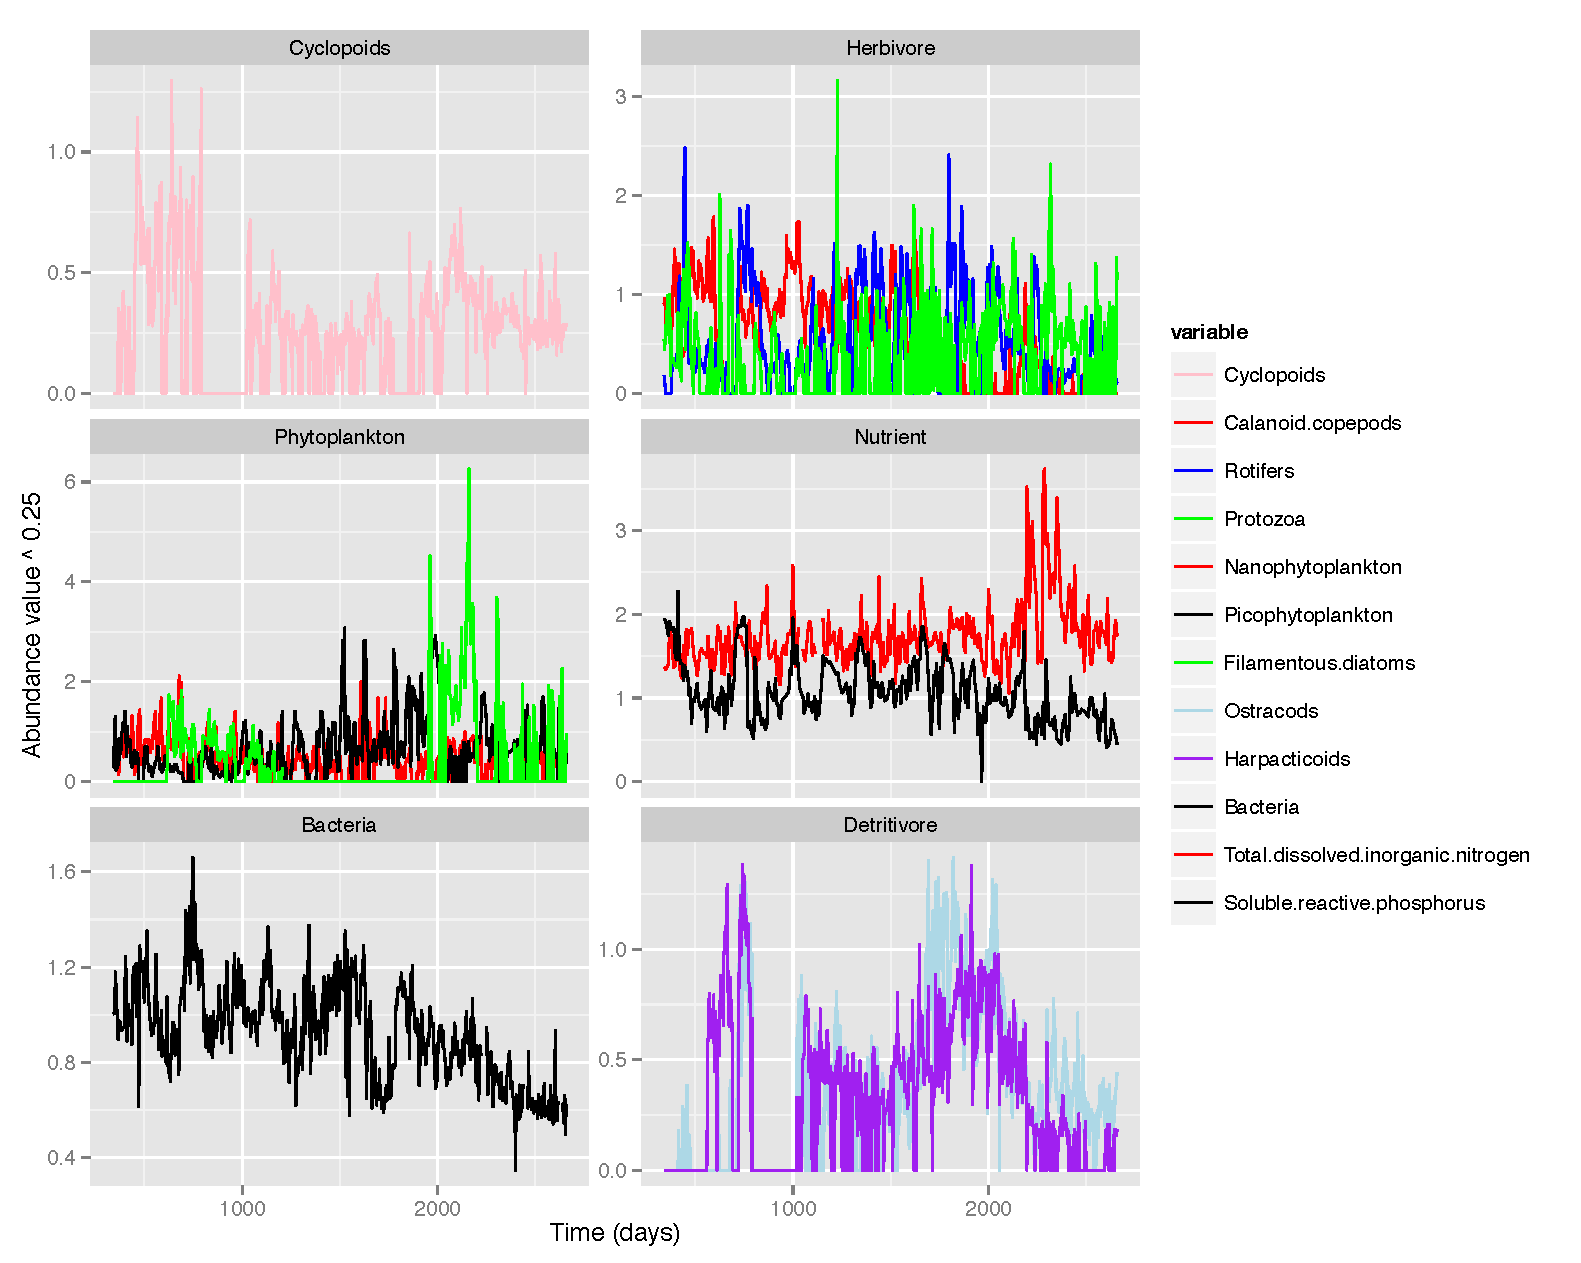
\includegraphics{figures/obs_pop_dyn.pdf}
\caption{\label{fig:dynamics}Observed population dynamics.}
\end{figure}

\subsection{Data transformations}\label{data-transformations}

The original publication states that long sequences of zeros were
removed from time series prior to transformation and further analysis.
We removed zeros by matching the removals to those in the transformed
version of the data in the published Excel file mentioned above.
Subsequent transformation steps were:

\begin{enumerate}
\def\labelenumi{\arabic{enumi}.}
\tightlist
\item
  Interpolation to create equally spaced observations in time series.
\item
  Fourth root transformation.
\item
  Detrending of five of the time series.
\item
  Rescaling to zero mean and unit standard deviation.
\end{enumerate}

The reproduced transformed data closely matched the published
transformed data (figure \ref{fig:trans_comp1}).

\begin{figure}[htbp]
\centering
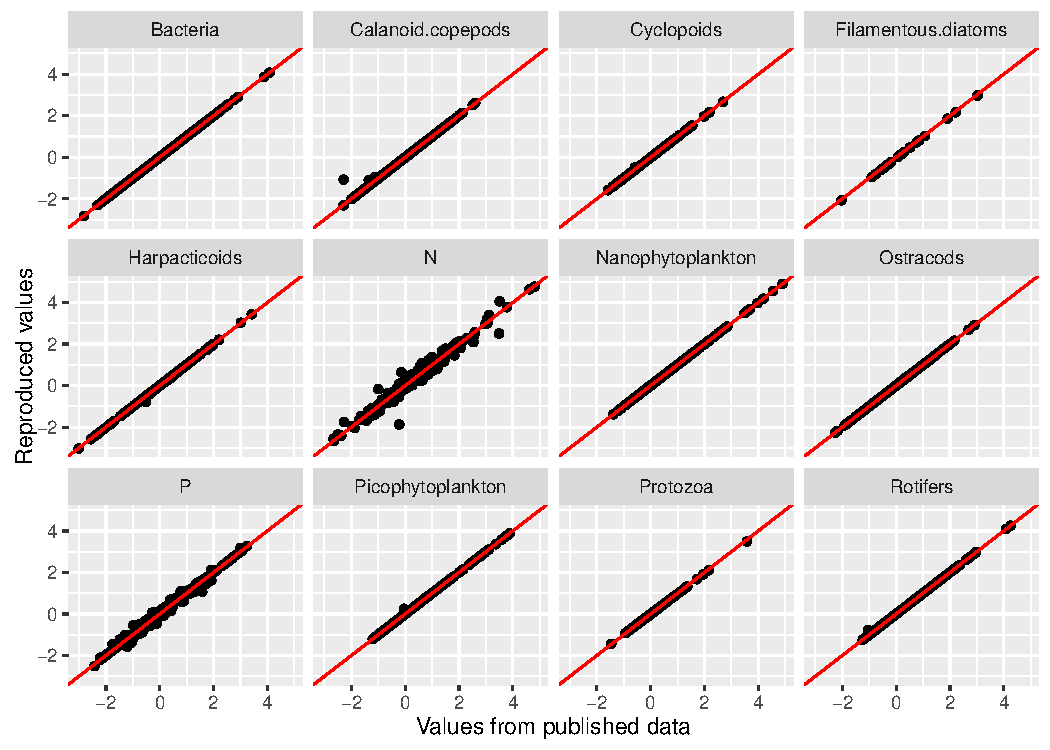
\includegraphics{figures/zero_rem_trans_comparison.pdf}
\caption{\label{fig:trans_comp1}Comparison of published transformed data
with reproduced transformed data. The red line is the 1:1 line.}
\end{figure}

\subsection{Correlations among species
abundances}\label{correlations-among-species-abundances}

Correlations among species abundances presented in Table 1 of the
original article closely matched our reproduced correlations, calculated
from the transformed data with zeros removed (figure
\ref{fig:corr_comp}). Deviations between the original and reproduced
correlations are relatively small and infrequent.

\begin{figure}[htbp]
\centering
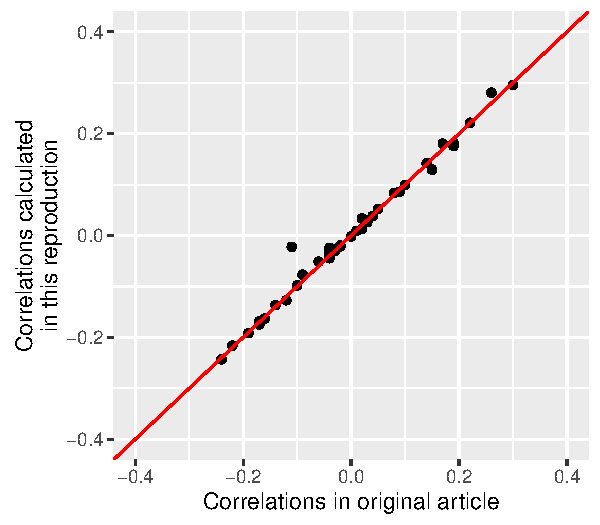
\includegraphics{figures/correlation_comparison.pdf}
\caption{\label{fig:corr_comp}Comparison of calculated correlations
among species abundances in the original article and this reproduction.}
\end{figure}

Highlighted in the text of the original paper were: negative
correlations of picophytoplankton with protozoa, and of
nanophytoplankton both with rotifers and calanoid copepods, positive
correlation of picophytoplankton with calanoid copepods, negative
correlation between bacteria and ostracods, and positive correlation
between bacteria and phosphorus. All of these correlations were at least
qualitatively reproduced.

\subsection{Spectral analyses}\label{spectral-analyses}

Spectral analyses in the original paper were presented graphically in
figures S3 (raw spectrograms) and S4 (Welch periodograms). The original
article states: ``fluctuations covered a range of different
periodicities'', and ``picophytoplankton, rotifers and calanoid copepods
seemed to fluctuate predominantly with a periodicity of about 30 days.''
Our reproduced spectra (not shown here, but code provided) were a
reasonably close match to the spectra in the original article.

\subsection{Lyapunov exponents by direct
method}\label{lyapunov-exponents-by-direct-method}

The original article states: ``the distance between initially nearby
trajectories increased over time, and reached a plateau after about
20--30 days''. The reproduced results (figure \ref{fig:divergence}) are
consistent with this statement. The original article also stated that
the analyses ``yielded significantly positive Lyapunov exponents of
strikingly similar value for all species (Fig. 3; mean exponent = 0.057
per day, s.d. = 0.005 per day, n = 9)''. Reproduced exponents had very
similar mean value, but had larger standard deviation (mean = 0.060 and
s.d. = 0.014), resulting from quantitative differences in reproduced
divergence rates (figure \ref{fig:divergence}) and therefore Lyapunov
exponents (figure \ref{fig:LE_comparison}).

\begin{figure}[htbp]
\centering
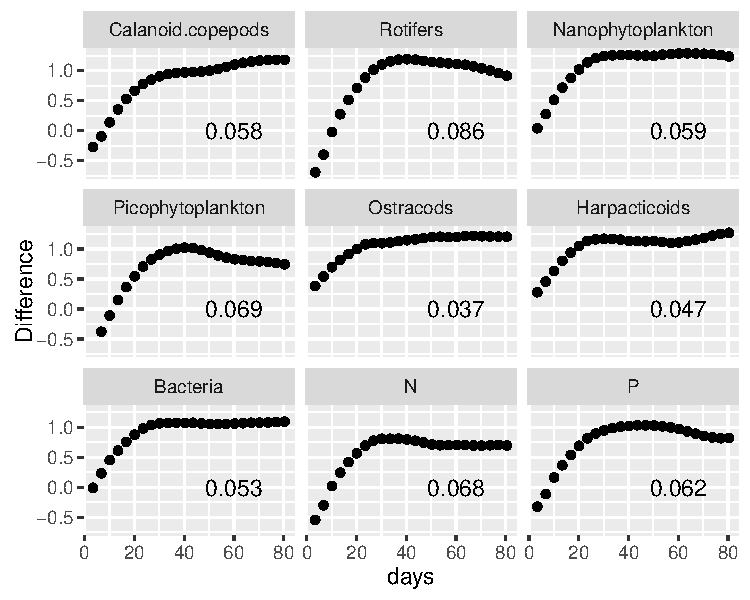
\includegraphics{figures/div_rate.pdf}
\caption{\label{fig:divergence}Reproduced divergence rates and Lyapunov
exponents (equivalent to figure 3 in the original article).}
\end{figure}

\begin{figure}[htbp]
\centering
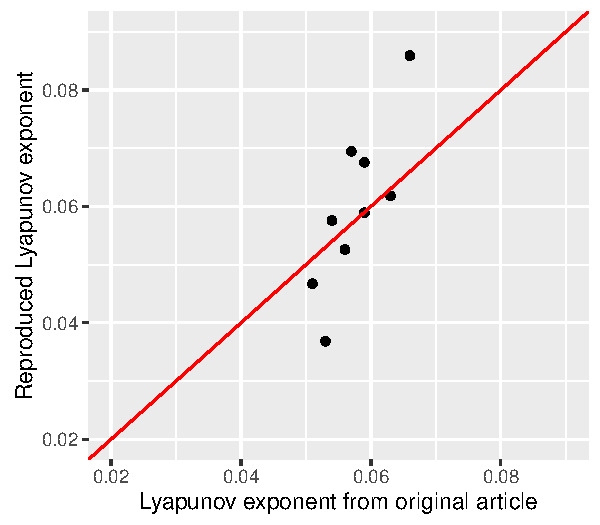
\includegraphics{figures/LE_comparison.pdf}
\caption{\label{fig:LE_comparison}Comparison of original and reproduced
directly estimated Lyapunov exponents.}
\end{figure}

\subsection{Lyapunov exponents by indirect
method}\label{lyapunov-exponents-by-indirect-method}

The data received directly from Stephen Ellner (file
`interp\_short\_allsystem\_newnames.csv' in the reproduction repository)
was interpolated, but without zeros removed. The reproduced interpolated
data, without zeros removed, matched closely this data (figure
\ref{fig:trans_comp2}).

\begin{figure}[htbp]
\centering
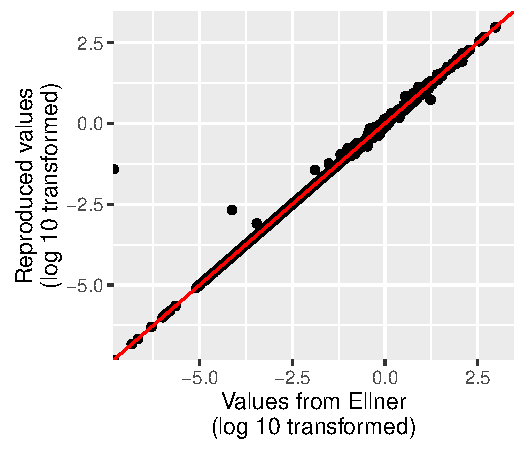
\includegraphics{figures/repro_ellner_comp.pdf}
\caption{\label{fig:trans_comp2}Comparison of interpolated data provided
by Ellner with reproduced interpolated data (no removal of zeros). The
red line is the 1:1 line.}
\end{figure}

The original paper reported a global Lyapunov exponent calculated via
two modelling approaches (neural network and generalised additive models
{[}GAMs{]}). Only the GAM approach was reproduced, with the assistance
of code donated by Stephen Ellner. The original article obtained a
global Lyapunov exponent of 0.08 per day. The reproduced value was 0.04.
We did not reproduce the bootstrapping used to give confidence intervals
around this estimate.

\subsection{Predictability decay}\label{predictability-decay}

The article stated: ``For short-term forecasts of only a few days, most
species had a high predictability of R2 = 0.70 -- 0.90 (Fig. 2).
However, the predictability of the species was much reduced when
prediction times were extended to 15--30 days.'' The reproduced
predictabilities, which were calculated from the GAMs, were consistent
with these qualitative statements, and were most often quantitatively
similar (\ref{fig:prediction_distance}). We did not reproduce the
predictability estimates for linear models.

\begin{figure}[htbp]
\centering
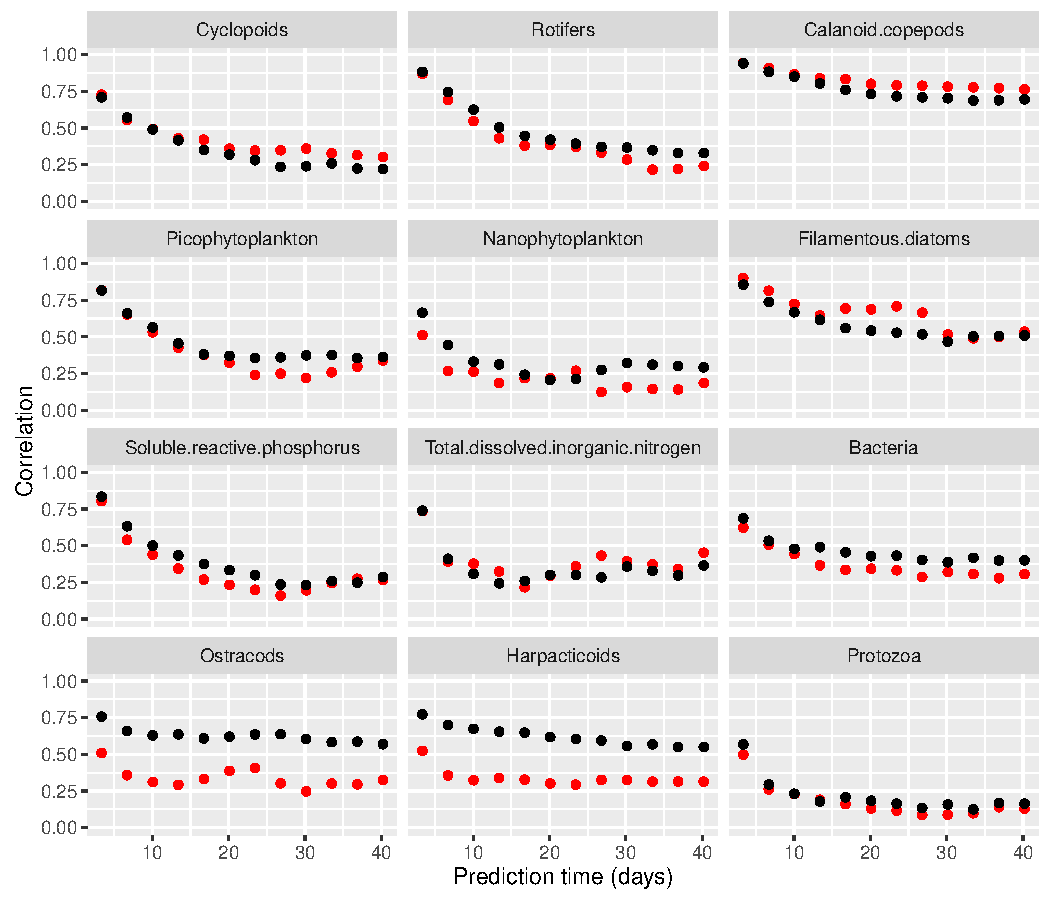
\includegraphics{figures/prediction_distance.pdf}
\caption{\label{fig:prediction_distance}Predictability (correlation
between predicted and observed abundances) and prediction distance
(days) (figure 2 in the original article). Reproducted data in red, and
data from original publication in black.}
\end{figure}

\section{Conclusion}\label{conclusion}

The reproduced results were qualitatively identical to those in the
original article, and therefore support the conclusion of chaotic
dynamics. For example, all Lyapunov exponents estimated by direct method
were positive, as in the original article. Quantitative differences may
have resulted from difference in algorithms used. For example, the
original used the
\href{http://www.mpipks-dresden.mpg.de/~tisean/}{Tisean software} to
calculate Lyapunov exponents. As this was available from CRAN
\href{http://cran.r-project.org/web/packages/RTisean/index.html}{until
mid 2014} and since it is a bit less well integrated with R, we instead
used the tseriesChaos package (\textcite{tseriesChaos}), which in any
case was largely inspired by the TISEAN project. In addition, there may
have been some difference in algorithm parameters, as not all parameters
required by the function we used were reported in the original ms.

Quantitative differences in predictability decay (figure
\ref{fig:prediction_distance}) remain unexplained, though could result
from original analyses using neural networks, and the reproduction using
GAMs. The difference in estimate of the global Lyapunov exponent (0.08
in the original article and 0.04 here) appears to be due to difference
in data used (illustrated in figure \ref{fig:trans_comp2}).

In conclusion, this reproduction supports the general scientific
conclusions of the original article, but also shows how difficult can be
an accurate quantitative reproduction, even in the presence of the
extensive methodological details provided alongside the original
article.

\section{Acknowledgements}\label{acknowledgements}

This reproduction was made as part of the Reproducible Research in
Ecology, Evolution, Behaviour, and Environmental Studies (RREEBES)
Course, lead by Owen Petchey at the University of Zurich. More
information about the course
\href{https://github.com/opetchey/RREEBES/blob/master/README.md}{here}
on github. Many thanks to Elisa Benincà, Stephen Ellner and Jef Huisman
for assistance, and to Stephen Ellner for providing unpublished data and
code.

{\sffamily \small
  \printbibliography[title=References]
}
\end{document}
